\documentclass[a4paper]{article}

%% Language and font encodings
\usepackage[english]{babel}
\usepackage[utf8x]{inputenc}
\usepackage[T1]{fontenc}

%% Sets page size and margins
\usepackage[a4paper,top=3cm,bottom=2cm,left=3cm,right=3cm,marginparwidth=1.75cm]{geometry}

%% Useful packages
\usepackage{amsmath}
\usepackage{amsfonts}
\usepackage{amssymb}
\usepackage{graphicx}
\usepackage[colorinlistoftodos]{todonotes}
\usepackage[colorlinks=true, allcolors=blue]{hyperref}

\title{\textbf{Teorema de muestreo de Nyquist-Shannon}}
\author{Jesús Joaquín Rojas, Rodolfo Pérez Ferro, María de Lourdes Oros Barrón.}
\date{Noviembre de 2016.}

\begin{document}
\sffamily
\maketitle

\section{\sffamily La transformada de Fourier.}
La transformada de Fourier transforma señales que dependen del tiempo en señales dependientes de la frecuencia. 
Tal herramienta ha sido de gran utilidad en ingeniería, física, ciencias de la computación y por supuesto se ha seguido desarrollando en matemáticas básicas. En esta era computacional, la transformada de Fourier ha sido de gran ayuda para el tratamiento digital de señales y audio, filtrado digital, resolución de ecuaciones en derivadas parciales, desarrollo de algoritmos de multiplicación rápida de grandes enteros, entre otros.\\
En este trabajo mostraremos un resultado de gran importancia en la teoría de la computación. Veremos que si conocemos el muestreo de una función en suficientes puntos, podemos recuperar exactamente a esta.\\

\subsection{\sffamily Transformada de Fourier y su inversa.}
Presentamos enseguida la transformada de Fourier en diferentes situaciones:\\
\begin{enumerate}
\item Dada una función $f\in L^{2}\mathbb{(R)},$ se define su transformada de Fourier como $$
\widehat{f}(\xi)=\int_{\mathbb{R}} \exp(-2\pi ix\xi)f(x)dx
$$ asi como su inversa
$$
f(x)=\int_{\mathbb{R}} \exp(2\pi i x\xi) \widehat{f}(\xi)d\xi.
$$
$x$ representa el tiempo y $\xi$ la frecuencia de $f.$
\\
\item Si $\{f_{n}\}_{n} \in l^{2}$ es una sucesión de funciones entonces la transformada de Fourier de tal sucesión es la función de periodo uno
$$
\widehat{f}(\xi)=\sum_{n=-\infty}^{\infty} \exp(-2i\pi n\xi)f_{n}
$$ con $f_{n}=\int\limits_{0}^{1}\exp(2i\pi n\xi) \widehat{f}(\xi)d\xi.$
\\
\item Si $f$ es una función de $x$ de periodo $1$, entonces los coeficientes de Fourier $f_{n}$ de $f$ para $n\in \mathbb{N}$ y la formula de inversión inversa son:
$$
\widehat{f_{n}}=\int_{0}^{1}f(x)\exp(-2\pi inx)dx
$$ y $$
f(x)=\sum_{n=-\infty}^{\infty} \widehat{f_{n}}\exp(2i\pi nx)
$$ respectivamente.
\\
\item Si $(f_{0},f_{1},...,f_{N})$ es una sucesión de funciones entonces su transformada discreta de Fourier así como su inversa son respectivamente:
$$
\widehat{f_{m}}=\frac{1}{\sqrt[]{N}}\sum_{n=0}^{N-1}\exp\left(-2\pi i\frac{nm}{N}\right)f_{n};
$$ $$
f_{m}=\frac{1}{\sqrt[]{N}}\sum_{n=0}^{N-1}\exp\left(2\pi i\frac{nm}{N}\right)\widehat{f_{n}}.
$$
\end{enumerate}

\subsection{\sffamily Algunas propiedades importantes.}
\begin{enumerate}
\item Isometría$\left \| f \right \|_{2}=\left \| \widehat{f} \right \|_{2}.$
\item Convolución $\widehat{fg}=\widehat{f} \ast \widehat{g}$ y $\widehat{f\ast g}=\widehat{f} \widehat{g}.$
\item Traslación $\widehat{f(x-a)}=\exp(-2\pi ia\xi)\widehat{f}$ y $\widehat{f}(\xi-a)=\widehat{\exp(-2\pi ia\xi)}f.$ 
\item Producto por escalar $\widehat{f(ax)}=\frac{1}{a}\widehat{f}(\frac{x}{a}).$
\item Cauchy: $\widehat{\exp(-2\pi |x|)}=\frac{1}{\pi(1+x^{2})}.$
\item Propiedad Gaussiana:
$$
\widehat{e^{\frac{-x^{2}}{2\sigma ^{2}}}}=\sqrt[]{2\pi}\sigma e^{-2\pi^{2}\sigma^{2}\xi^{2}}.
$$
\\
\item En el procesamiento de señales se utiliza la relación de autocorrelación y el espectro potencia.\\ 
La autocorrelación está dada por:
$$
f \ast f(-x)= \int f(y)f(y-x)dy
$$ y con ello $$
\widehat{(f \ast f^{-1})}=|\widehat{f}|^{2}.
$$
\\

\end{enumerate}

\section{\sffamily Teorema de muestreo de Nyquist-Shannon}
\subsection{\sffamily El teorema de muestreo}
Sea $f\in$ $L^{2}(\mathbb{R})$ una función limitada a una banda, esto es, existe $W > 0$ tal que su transformada de Fourier $\widehat{f}$ es cero fuera de $[-W,W],$ i.e. $$
Support(\widehat{f}) \subset [-W,W].
$$
Entonces $f$ puede ser recuperada a partir de sus muestras en los puntos $\frac{n}{2W}$ para $n\in \mathbb{N}$ vía interpolación como sigue:
$$
f(t)=\sum_{n\in \mathbb{N}} f\left(\frac{n}{2W}\right)\frac{\sin(\pi(2Wt-n))}{\pi(2Wt-n)},$$ 
$\forall t\in \mathbb{R}.$\\
\\
Lo anterior nos dice que podemos recuperar la función siempre y cuando la frecuencia de muestreo sea superior al doble de la máxima frecuencia a muestrear.
\\
Demostración:\\
\\
\\
Recordemos que dada una función $f,$ su transformada de Fourier se define como:
$$
\widehat{f}(\xi)=\int_{\mathbb{R}} \exp(-2\pi ix\xi)f(t)dt.
$$
\\
Supongamos que existe $W>0$ tal que $Support(\widehat{f})\subset [-W,W].$\\
\\
Definamos $F:[-\frac{1}{2},\frac{1}{2}]\rightarrow \mathbb{R}$ la función $F(x)=\widehat{f}(2Wx).$\\
\\
La función $F$ es una función definida en los reales y es de periodo $1$, por lo que podemos escribirla mediante la transformada de Fourier como sigue: 
$$
F(x)=\sum_{n=-\infty}^{\infty}C_{n}\exp(-2i\pi nx)
$$ donde $C_{n}=\int_{-1/2}^{1/2}F(x)\exp\left(2i\pi nx\right)=\int_{-1/2}^{1/2}\widehat{f}(2Wx)\exp\left(2i\pi nx\right).$\\
(El anterior es el caso 3.)
\\
\\
Haciendo el cambio de variable $\xi=2Wx$ se tiene que $d\xi=2Wdx.$
Luego \\
\begin{eqnarray*}
	C_{n}
	&=& \int\limits_{-1/2}^{1/2} \widehat{f}(\xi)\exp\left(2\pi in\frac{\xi}{2W}\right)\frac{1}{2W}d\xi \\
	&=& \frac{1}{2W}\int\limits_{-1/2}^{1/2} \widehat{f}(\xi)\exp\left(2\pi in\frac{\xi}{2W}\right)d\xi \\
    &=& ^{(*)} \frac{1}{2W}f\left(\frac{n}{2W}\right).
\end{eqnarray*}
\\
En la igualdad $(*)$ recordemos que como \\
$$f(x)=\int_{\mathbb{R}}\exp(2\pi ix\xi)\widehat{f}(\xi)d\xi=\int\limits_{-1/2}^{1/2} \exp\left(2\pi ix\xi\right)\widehat{f}(\xi)d\xi$$ entonces: \\
$$f\left(\frac{n}{2W}\right)=\int\limits_{-1/2}^{1/2} \widehat{f}(\xi)\exp\left(2\pi i\frac{n}{2W} \xi\right)d\xi.$$\\
\\
Así $
C_{n}=\frac{1}{2W}f\left(\frac{n}{2W}\right)
$ para toda $n.$\\

Usando ahora la formula de inversi\'on
con la transfomada de Fourier y el hecho de que esta tiene soporte en $[-W,W]$ tenemos
\begin{eqnarray*}
 f(t)
 &=& \int_{-\infty}^{\infty}{e^{2\pi i t \xi} \hat{f}(\xi) d\xi}\\
 &=& \int_{-W}^{W}{e^{2\pi i t \xi} \hat{f}(\xi) d\xi}\\
 &=& \int_{-1/2}^{1/2}{e^{4\pi i t W x} \hat{f}(2Wx) 2W dx}\\
 &=& \int_{-1/2}^{1/2}{e^{4\pi i t W x} F(x) 2W dx}\\
 &=& \int_{-1/2}^{1/2}{ e^{4\pi i t W x} 2W  \Big( 
 \sum_{n\in\mathbb{Z}}{ \frac{1}{2W} f\big(\frac{n}{2W}\big) e^{-2i\pi n x} }
 \Big)dx}\\
 &=& \sum_{n\in\mathbb{Z}}{  f\Big(\frac{n}{2W}\Big)
      \int_{-1/2}{1/2}^{ e^{2\pi i x(2Wt-n)} dx } }
\end{eqnarray*}
Expresemos la exponencial en t\'erminos de senos y consenos, y calculemos por separado la la integral
de la parte real y la de la parte compleja. La integral de la parte compleja se anula por ser seno
una funci\'on impar. Para la integral de la parte real tenemos
\begin{eqnarray*}
  \int_{-1/2}^{1/2}{cos(2\pi x A_n)}
  &=&\frac{sen(2\pi x A_n)}{2\pi A_n}\Big|_{-1/2}^{1/2}\\
  &=&\frac{sen(\pi A_n)-sen(-\pi A_n)}{2\pi A_n}\\
  &=& \frac{sen(\pi A_n)}{\pi A_n}
\end{eqnarray*}
Donde $A_n=2Wt-n$. Luego 
\begin{equation*}
 f(t)=\sum_{n\in\mathbb{Z}}{  f\Big(\frac{n}{2W}\Big) \frac{sen\big(\pi(2Wt-n)\big)}{\pi(2Wt-n)} }. 
\end{equation*}
$\Box$

\subsection{\sffamily Interpretación y \textit{Aliasing}}
El teorema nos da explícitamente la cota inferior de puntos que requerimos tomar de una señal para tener una buena buena discretización, donde podemos entender como buena discretización a aquella en la que la reconstrucción a la hora de aplicar la transformación genera la señal original.\\

\noindent De esta interpretación, tenemos lo siguiente: \textit{Para reconstruir una señal, debemos muestrear en una proporción mayor que el doble del componente más alto de frecuencia.}\\

\begin{center}
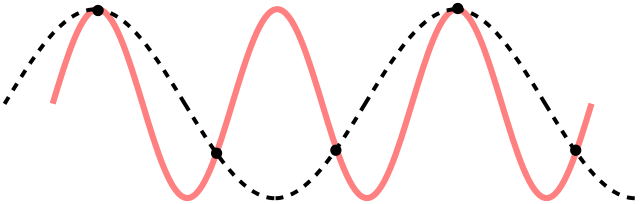
\includegraphics[width=0.5\textwidth]{curve1}\\
\textsc{Figura 1. Fucnión coseno y un muestreo de dicha función.}
\end{center}

\noindent En la \textsc{Figura 1} podemos darnos cuenta de que si muestreáramos dicha señal tomando en un periodo constante los puntos negros, al reconstruir obtendríamos la curva punteada, que es diferente a la señal original.\\

\noindent Cuando se muestrea de manera tal que de la reconstrucción no resulta la señal original se presenta un fenómeno conocido como \textit{aliasing}. Dicho fenómeno puede percibirse intuitivamente como irregularidades en la geometría.\\

\noindent Consideremos el siguiente ejemplo para entender mejor esta irregularidad geométrica (\textit{aliasing}) derivada del muestreo. Al graficar la función $f(x, y) = \cos(\alpha x + \beta y)$ en la rejilla $[0,200]\times[0,200]$, con $\alpha = 0.2$, $\beta = 0.4$ tenemos los siguientes resultados para diferentes $N$ (número de puntos en la rejilla, es decir, nuestro muestreo).\\

\begin{center}
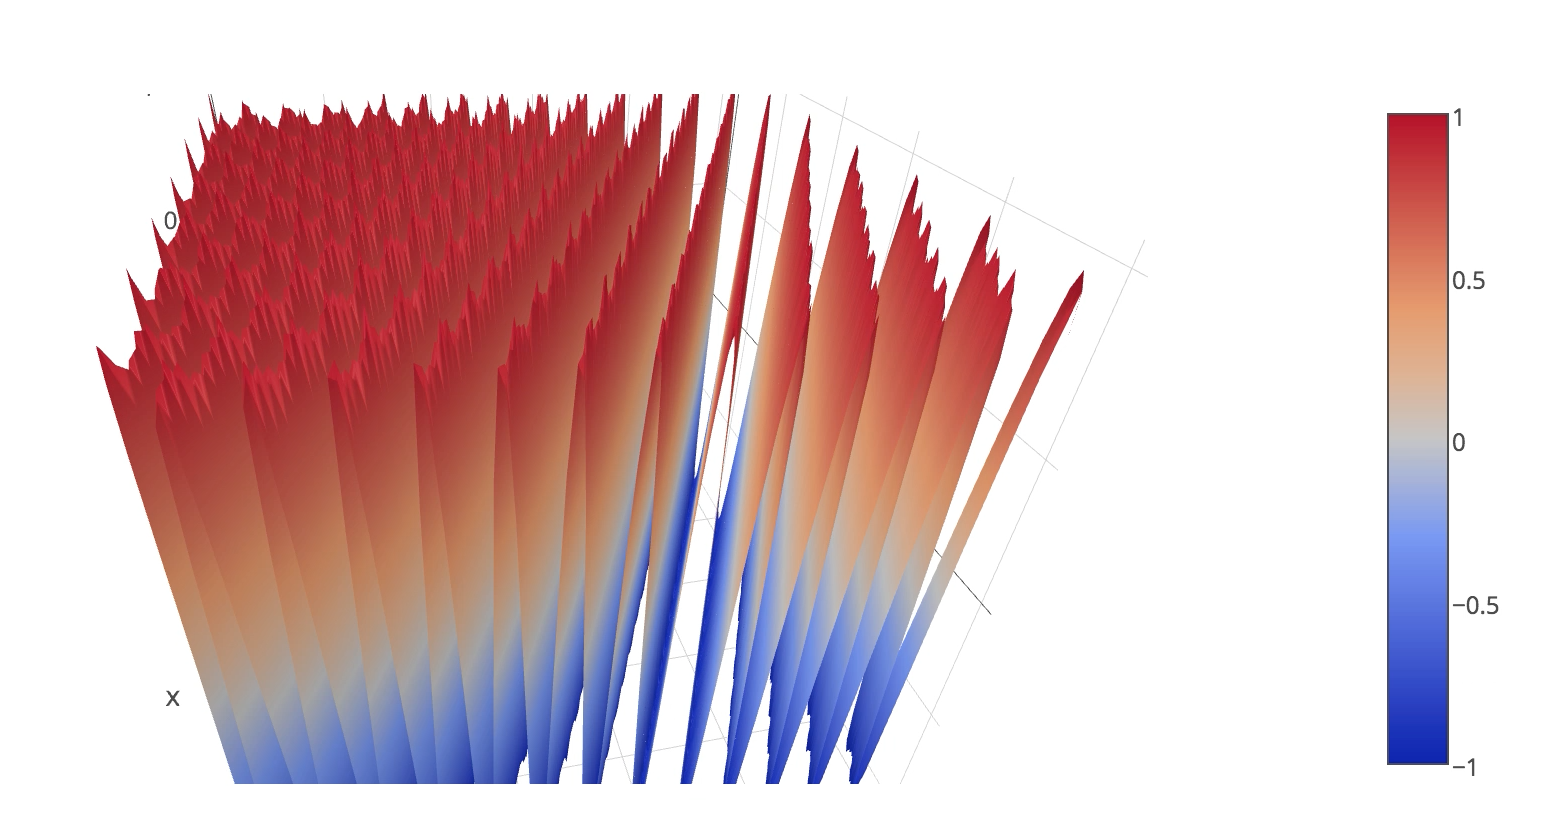
\includegraphics[width=0.5\textwidth]{g1}\\
\textsc{Figura 2. Gráfica de $f(x, y) = \cos(\alpha x + \beta y)$ con \\$N = (200\times 200)/2$, $\alpha = 0.2$ y $\beta = 0.4$.}
\end{center}
En la \textsc{Figura 2} podemos apreciar que precisamente al evaluar la función en una muestra de la mitad de puntos en la rejilla se presenta una irregularidad geométrica en la gráfica, teniendo picos.\\

\begin{center}
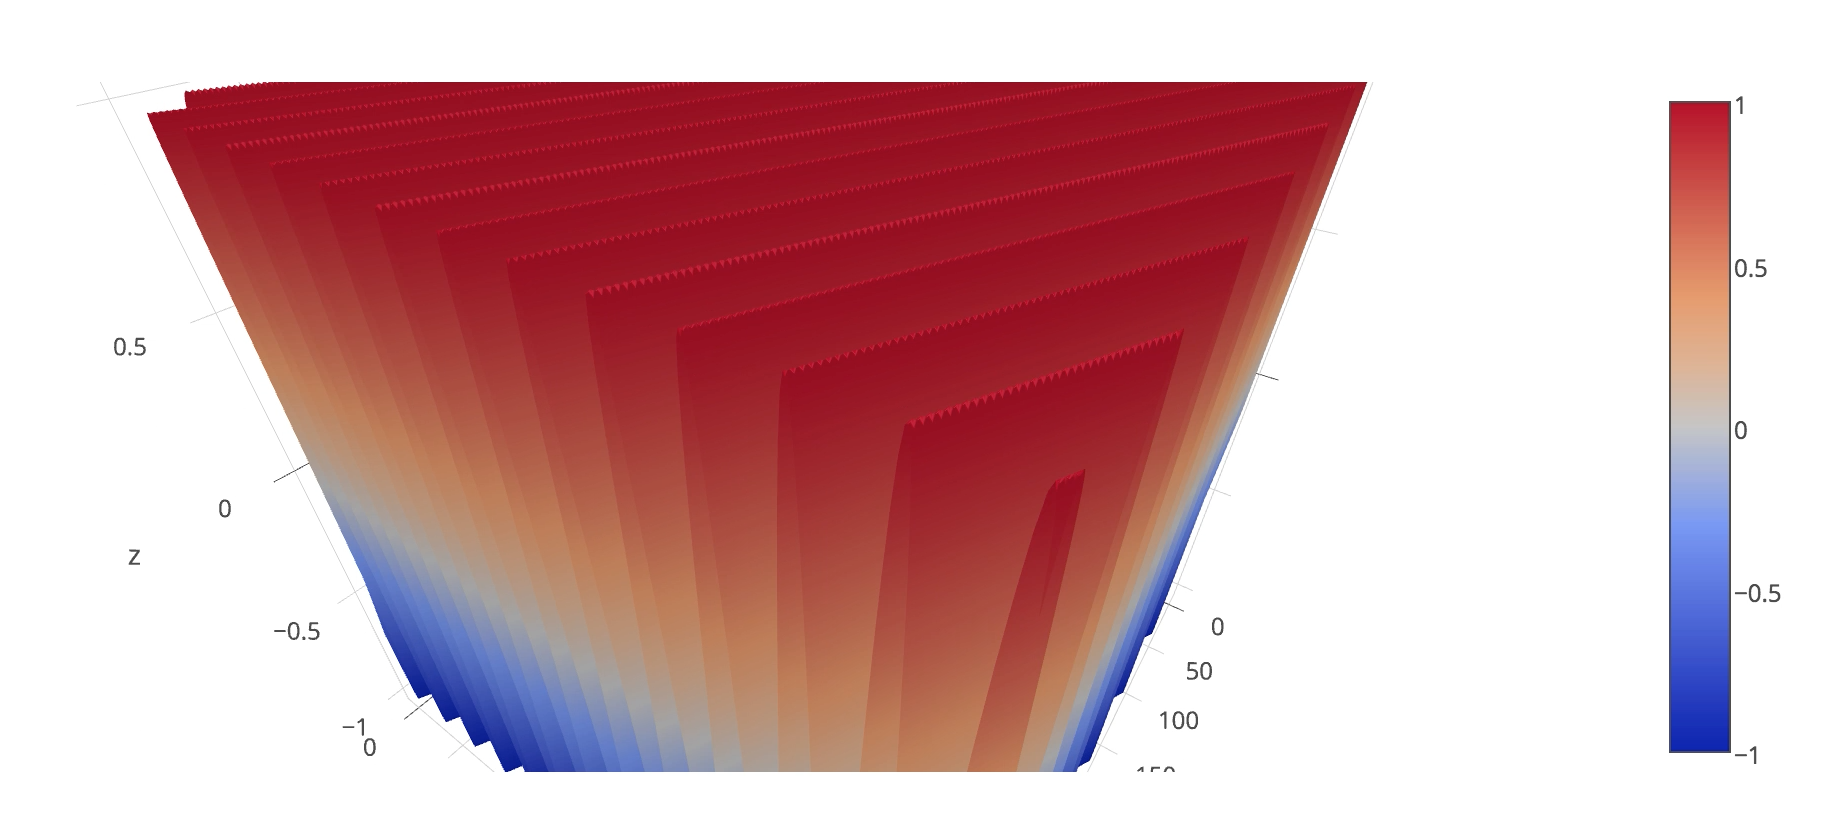
\includegraphics[width=0.5\textwidth]{g2}\\
\textsc{Figura 3. Gráfica de $f(x, y) = \cos(\alpha x + \beta y)$ con \\$N = 2(200\times 200)$, $\alpha = 0.2$ y $\beta = 0.4$.}
\end{center}
Al tomar justamente el doble de puntos muestra en la rejilla y evaluando la función, notamos que en la \textsc{Figura 3} se perciben menos las irregularidades, sin embargo siguen estando presentes.\\

\begin{center}
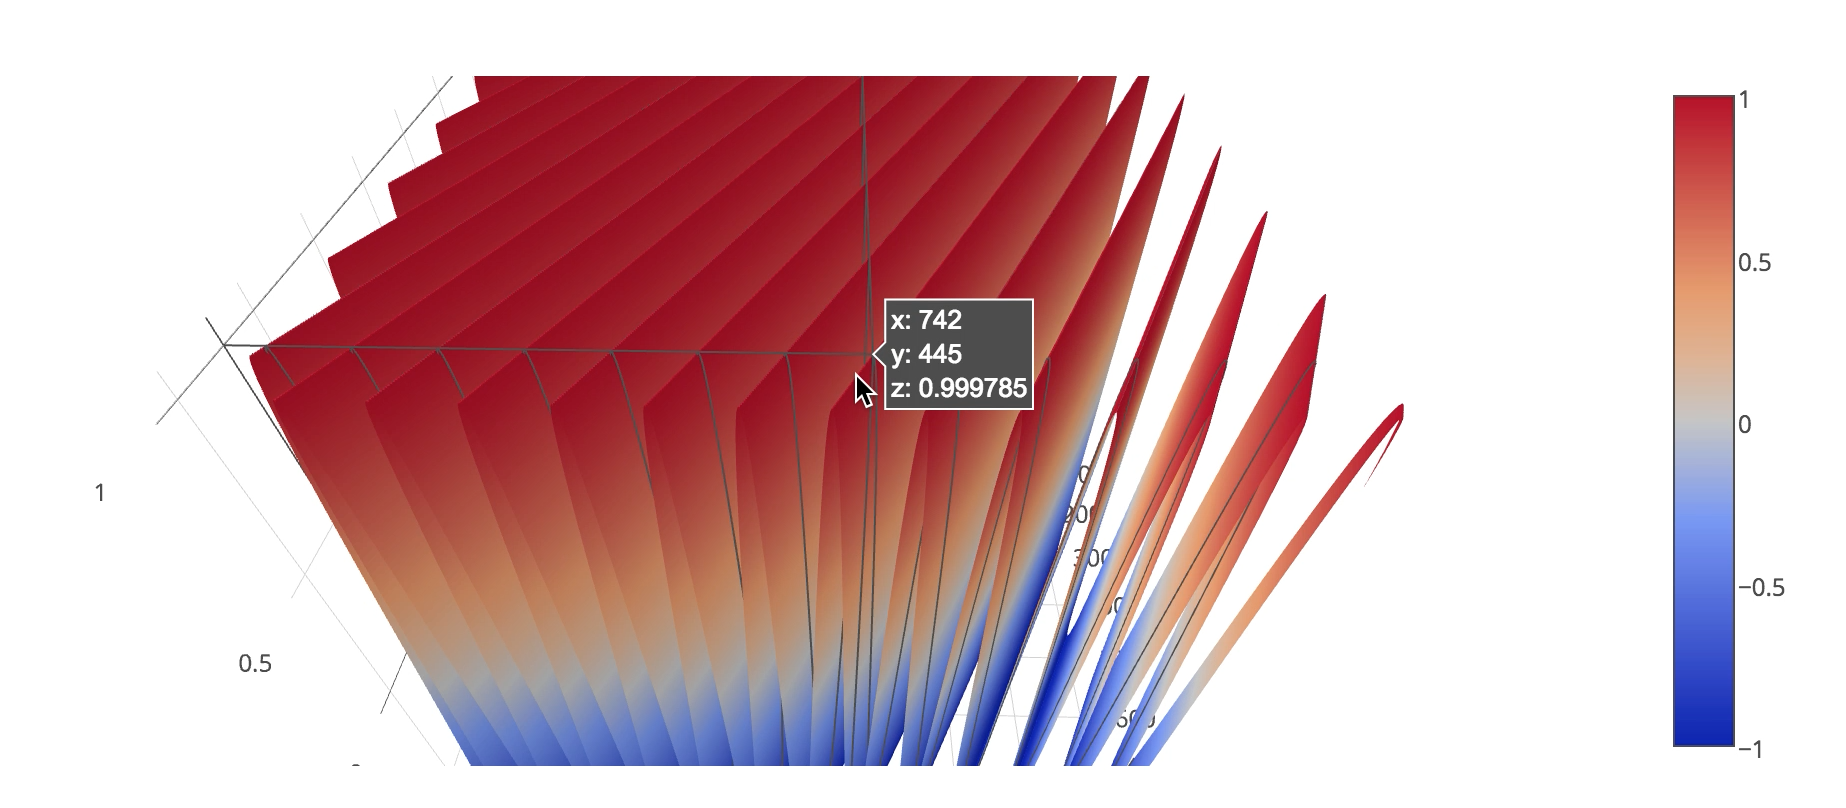
\includegraphics[width=0.5\textwidth]{g3}\\
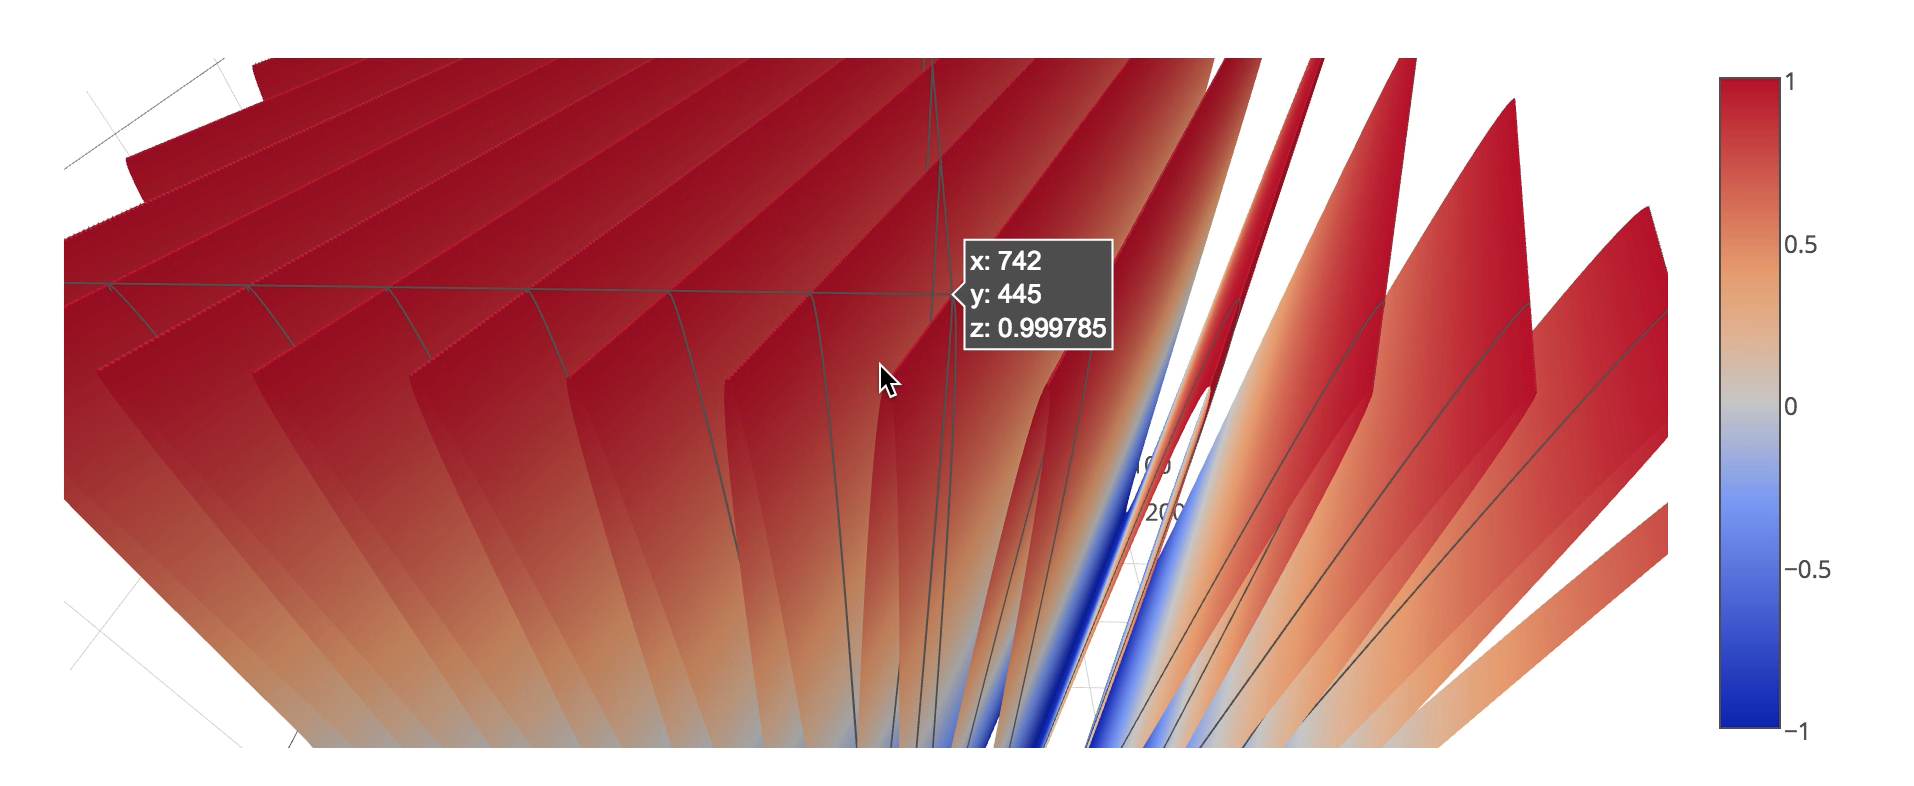
\includegraphics[width=0.5\textwidth]{g4}\\
\textsc{Figura 4. Gráfica de $f(x, y) = \cos(\alpha x + \beta y)$ con \\$N = 4(200\times 200$), $\alpha = 0.2$ y $\beta = 0.4$.}
\end{center}
Al tomar el cuádruple de puntos muestra en la rejilla y evaluando la función en la \textsc{Figura 4}, notamos que las irregularidades geométricas son casi imperceptibles.\\

\section{\sffamily Observaciones}
\begin{itemize}
\item El teorema demuestra que la reconstrucción exacta de una señal periódica continua en banda a partir de sus muestras, es matemáticamente posible si la señal está limitada en banda y la tasa de muestreo es superior al doble de su ancho de banda.

\item El fenómeno de \textit{aliasing} se presenta comunmente en gráficos por computadora:
\begin{center}
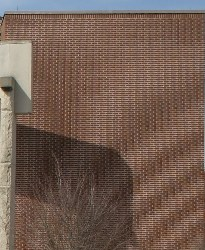
\includegraphics[width=0.45\textwidth]{bricks1}
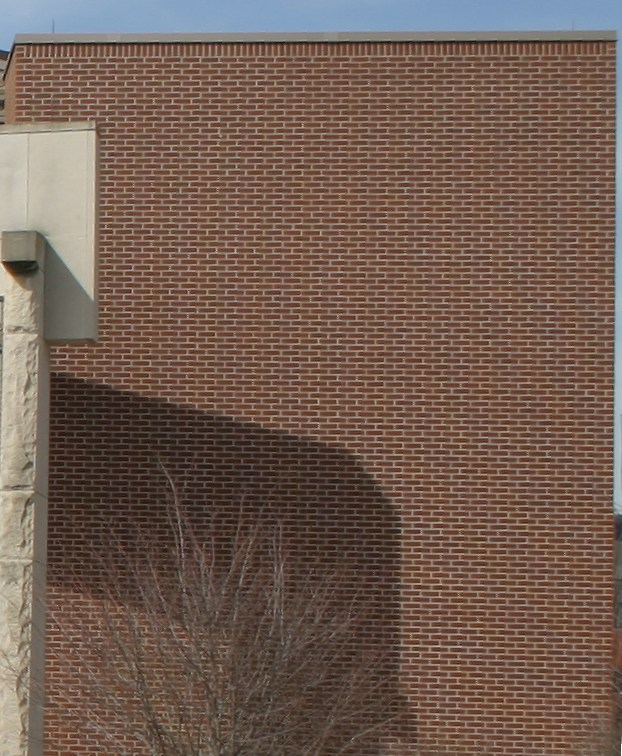
\includegraphics[width=0.45\textwidth]{bricks2}\\
\textsc{Figura 5. a) Fenómeno de aliasing en una imagen digital \\b) Muestreo correcto de la imagen.}
\end{center}
Para resolver dicho problema se utilizan comunmente filtros en las imágenes.
\end{itemize}
\end{document}